\documentclass{article}

\usepackage{graphicx}
\usepackage{tikz}
\usepackage{tikzsymbols}
\usetikzlibrary{calc,patterns,shapes.geometric}
\pagestyle{empty}
\usepackage[margin=0pt]{geometry}
\geometry{papersize={14in,12in}}

\def\centerarc[#1](#2)(#3:#4:#5){\draw[#1] ($(#2)+({#5*cos(#3)},{#5*sin(#3)})$) arc (#3:#4:#5);}

\begin{document}
	\begin{figure}
		\centering
		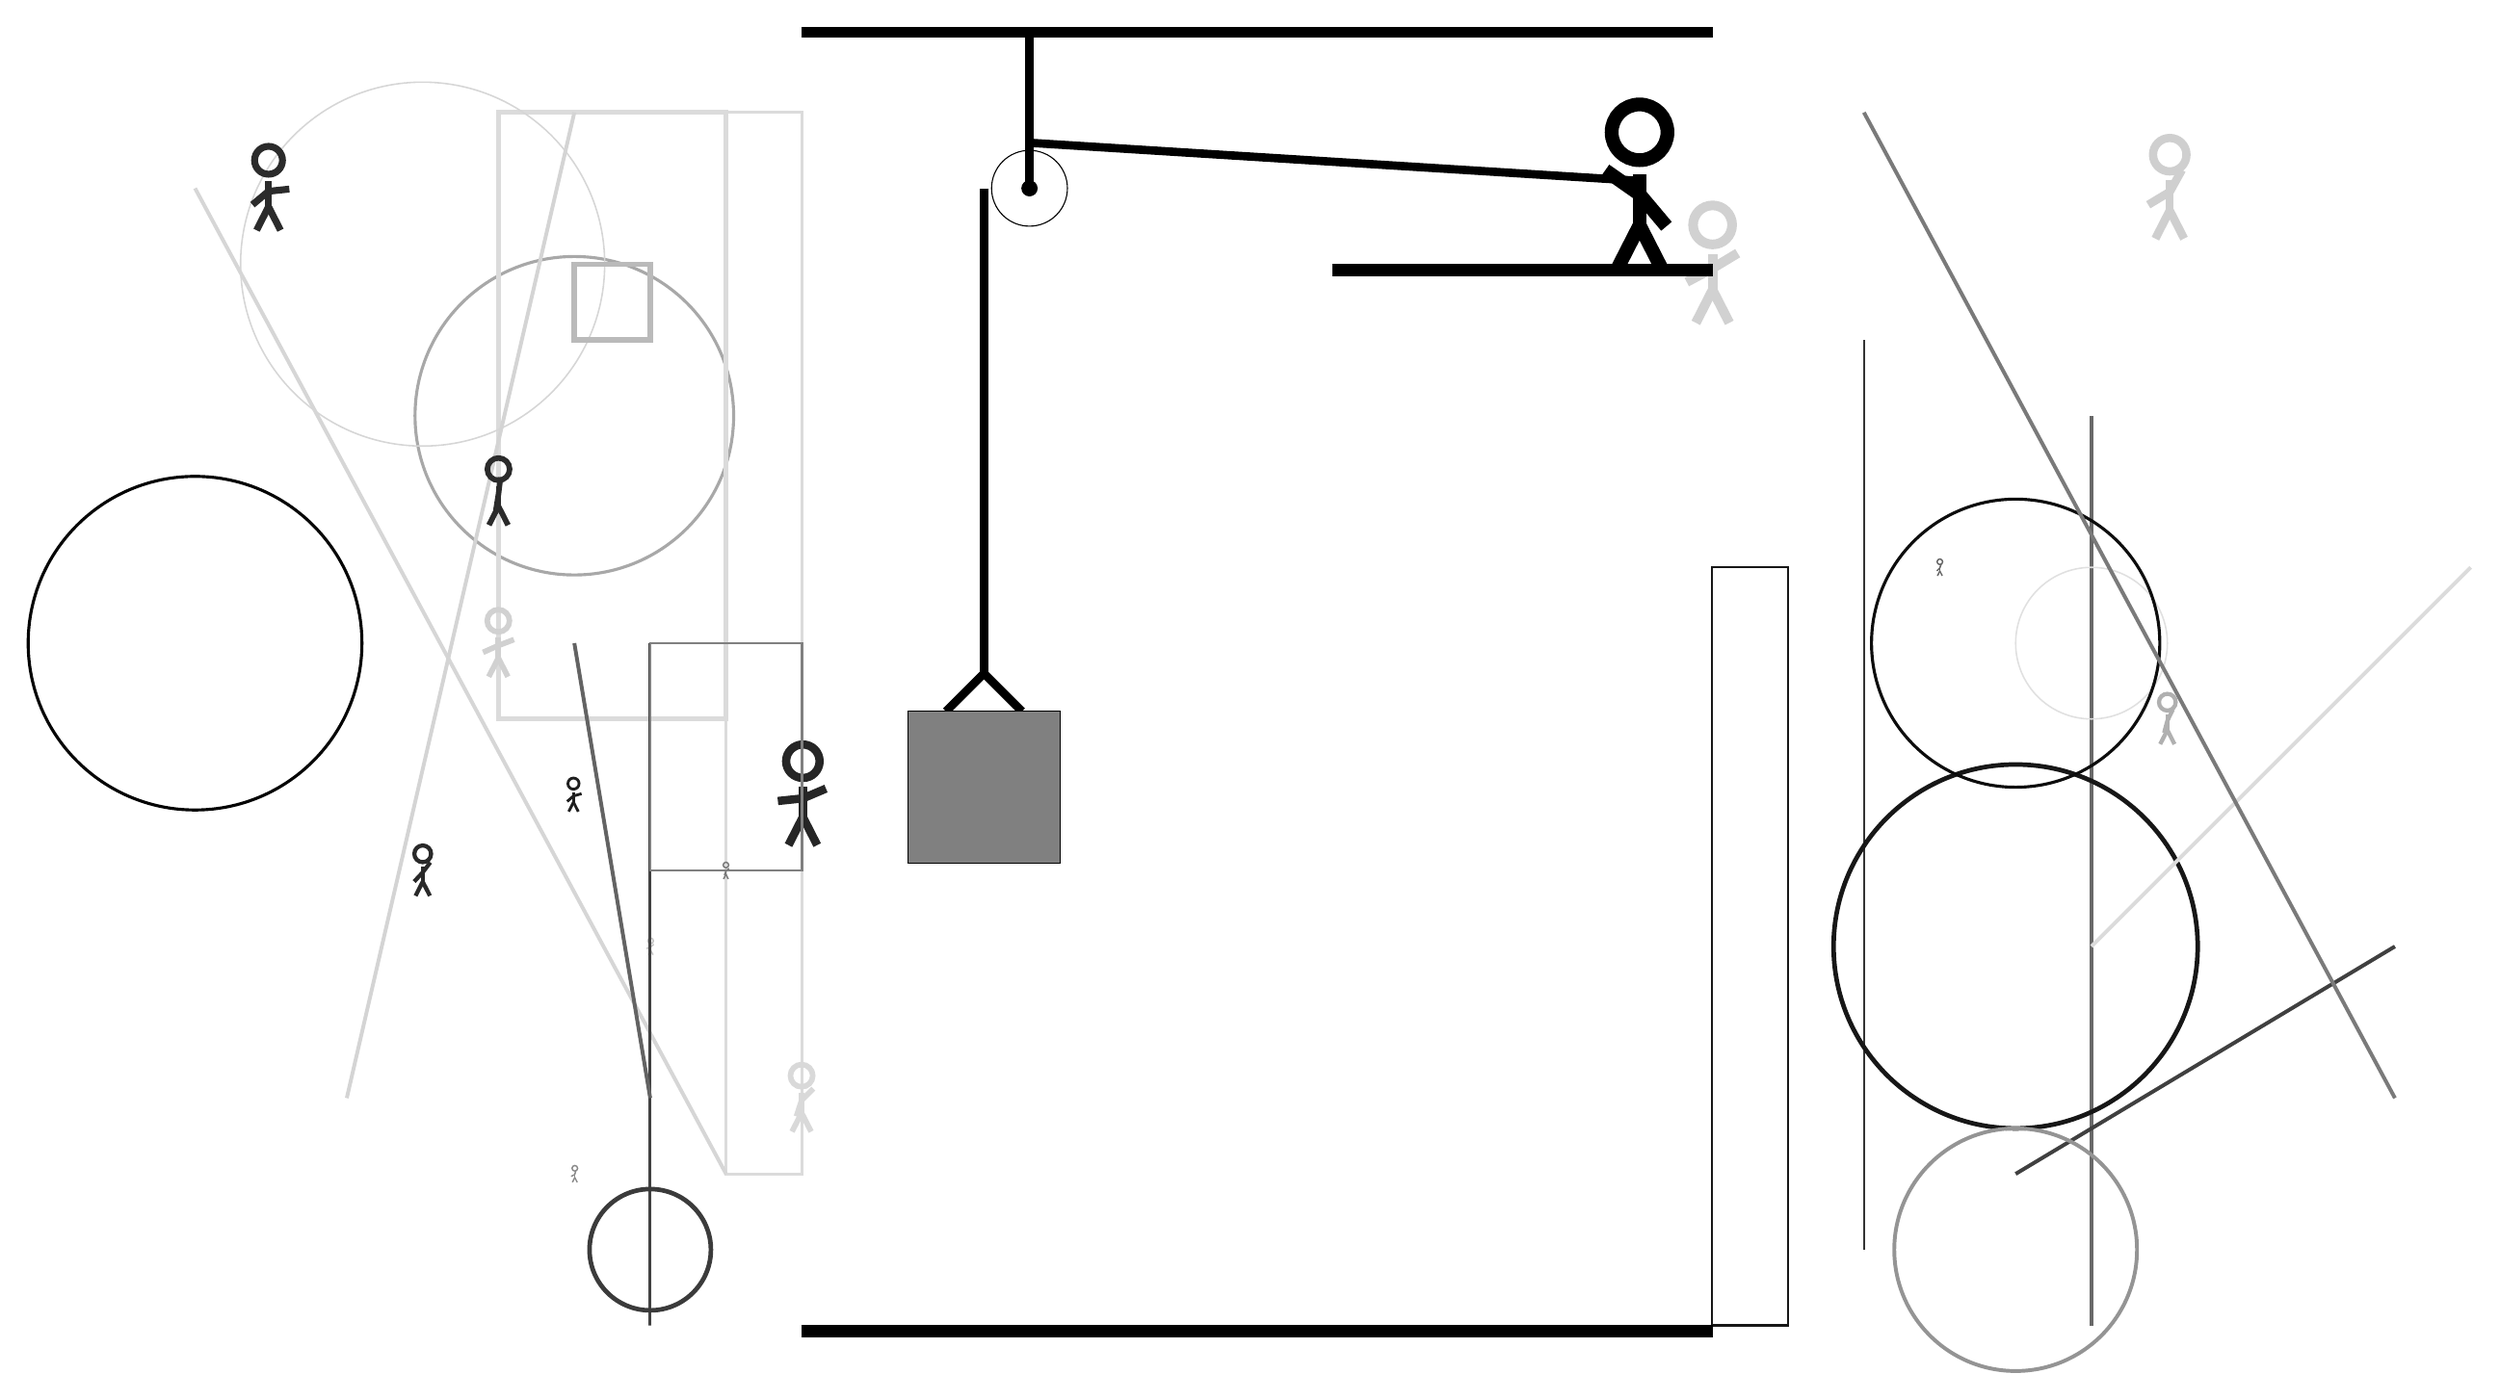
\begin{tikzpicture}
			%%%%% START %%%%%
			
			\draw[fill=black] (-2, 14) rectangle (10, 14.125);
			
			\draw (1, 12) circle (0.5);
			\draw[fill=black] (1, 12) circle (0.1);
			\draw[line width=1.1mm] (1, 14) -- (1, 12);
			
			\draw[line width=1.1mm](-0.1, 5.1) --  (0.4, 5.6) -- (0.9, 5.1);
			\draw[fill=black!50] (-0.6, 5.1) rectangle (1.4, 3.1);
			
			\draw[line width=0.4mm, color=black!14] (-2, 13) rectangle (-3, -1);
			
			\draw[line width=0.5mm, color=black!59](15, -3) -- (15, 9);
			\node[line width=0.2mm, color=black!25] at (-4, 2) {\Strichmaxerl[1][21][42]};
			\draw[line width=0.2mm, color=black!80] (12, 10) rectangle (12, -2);
			\node[line width=0.4mm, color=black!31] at (16, 5) {\Strichmaxerl[3][75][64]};
			\draw [line width=0.6mm, color=black!91](14, 2) circle (2.4);
			\draw[line width=0.5mm, color=black!16](-3, -1) -- (-10, 12);
			
			\draw [line width=0.4mm, color=black!34](-5, 9) circle (2.1);
			\draw[line width=0.5mm, color=black!75](14, -1) -- (19, 2);
			\draw[line width=0.6mm, color=black!14] (-3, 5) rectangle (-6, 13);
			\draw [line width=0.2mm, color=black!12](15, 6) circle (1.0);
			\node[line width=0.2mm, color=black!18] at (-6, 6) {\Strichmaxerl[4][24][21]};
			\draw [line width=0.4mm, color=black!95](14, 6) circle (1.9);
			
			\node[line width=0.4mm, color=black!84] at (-7, 3) {\Strichmaxerl[3][47][53]};
			\draw [line width=0.4mm, color=black!98](-10, 6) circle (2.2);
			\draw [line width=0.2mm, color=black!16](-7, 11) circle (2.4);
			\node[line width=0.7mm, color=black!85] at (-2, 4) {\Strichmaxerl[6][6][23]};
			
			\node[line width=0.3mm, color=black!53] at (-3, 3) {\Strichmaxerl[1][68][43]};
			\draw[line width=0.5mm, color=black!14](15, 2) -- (20, 7);
			\draw[line width=0.4mm, color=black!74] (-4, -3) rectangle (-4, 6);
			\draw[line width=0.3mm, color=black!91] (11, -3) rectangle (10, 7);
			
			\draw [line width=0.5mm, color=black!42](14, -2) circle (1.6);
			\draw[line width=0.3mm, color=black!50] (-4, 6) rectangle (-2, 3);
			\node[line width=0.7mm, color=black!60] at (13, 7) {\Strichmaxerl[1][45][71]};
			\draw[line width=0.5mm, color=black!52](12, 13) -- (19, 0);
			\node[line width=0.5mm, color=black!88] at (-5, 4) {\Strichmaxerl[2][41][16]};
			
			\draw[line width=0.7mm, color=black!27] (-4, 10) rectangle (-5, 11);
			\node[line width=0.6mm, color=black!18] at (10, 11) {\Strichmaxerl[7][28][31]};
			\draw[line width=0.5mm, color=black!17](-5, 13) -- (-8, 0);
			\node[line width=0.7mm, color=black!46] at (-5, -1) {\Strichmaxerl[1][27][76]};
			\node[line width=0.7mm, color=black!19] at (16, 12) {\Strichmaxerl[6][31][61]};
			
			\draw[line width=0.5mm, color=black!61](-5, 6) -- (-4, 0);
			\node[line width=0.4mm, color=black!83] at (-6, 8) {\Strichmaxerl[4][81][83]};
			\node[line width=0.4mm, color=black!15] at (-2, 0) {\Strichmaxerl[4][72][45]};
			
			\draw [line width=0.6mm, color=black!77](-4, -2) circle (0.8);
			\node[line width=0.7mm, color=black!83] at (-9, 12) {\Strichmaxerl[5][40][6]};
			
			\draw[line width=1.1mm](0.4, 12) -- (0.4, 5.6);
			\centerarc[line width=1.1mm](1, 12)(90:180:0.6)
			\draw[line width=1.1mm](1, 12.6) -- (9, 12.1);
			
			\node at (9, 12) {\Strichmaxerl[10][-35][-50]};
			\draw[fill=black] (5, 11) rectangle (10, 10.85);
			
			\draw[fill=black] (-2, -3) rectangle (10, -3.15);
			
			%%%%% END %%%%%
		\end{tikzpicture}
	\end{figure}	
\end{document}